\documentclass{article}
\title{CSCI 447 Project 2 Design Document}
\author{George Engle, Troy Oster, Dana Parker, Henry Soule}
\usepackage{hanging}
\usepackage{graphicx}
\begin{document}
\maketitle
\section{Introduction}
For this assignment, we are required to assess the performance of five different algorithms on six different data sets. The five algorithms used are $k$-nearest neighbors, edited $k$-nearest neighbors, condensed $k$-nearest neighbors, $k$-means clustering, and $k$-medoids clustering.  The essential purpose of the latter four algorithms is to produce a reduced data set with which to run k-nearest neighbors. We have found literature suggesting improved accuracy among nearest neighbor algorithms that employ data reduction [1][2].  Based on this, we have hypothesized that the average accuracy of $k$-nearest neighbors across all six data sets without reduction will be worse than the average accuracy across the six data sets once reduction has been performed via edited k-nearest neighbors, condensed k-nearest neighbors, k-means clustering, and k-medoids clustering.
%Possible TODO: add in description of loss functions we are using to define 'accuracy'.
\section{Experimental Design}

\begin{center}
    \makebox[\textwidth]{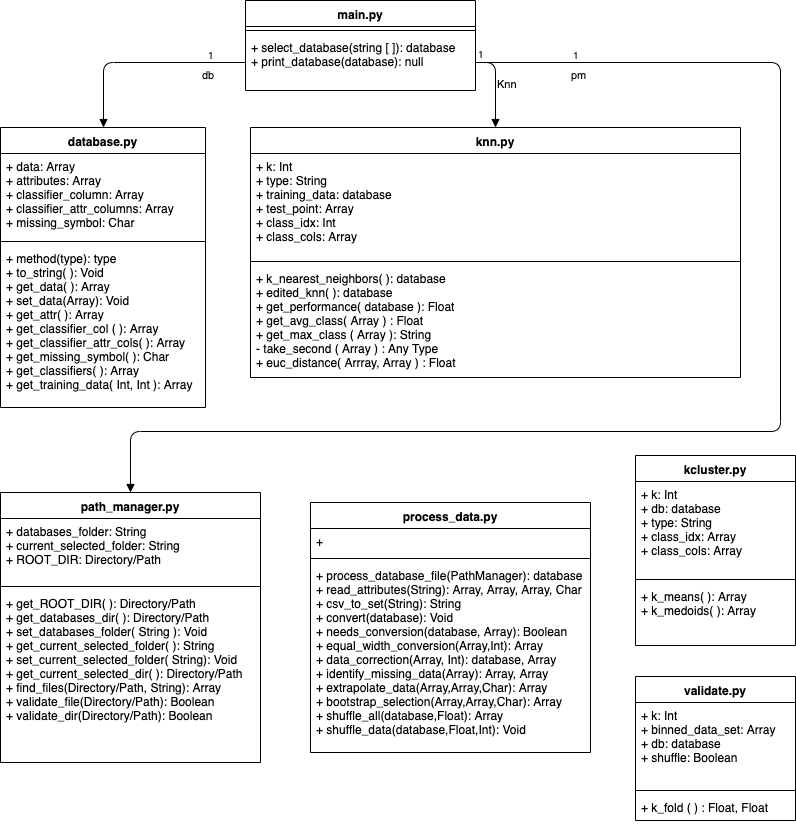
\includegraphics[width=4.75in]{uml}}
\end{center}


\subsection*{Components}
Our design has 5 primary components. $database.py$ is a wrapper class that will handle all functionality of each data set. Each instance of the database class will store the processed data of one our six data sets, the the index of the class attribute of its respective database. $knn.py$ will store our implementations of $k$-nearest neighbors, edited $k$-nearest neighbors, and condensed $k$-nearest neighbors. $kcluster.py$ will store the implementation of both clustering algorithms--$k$-means and $k$-medoids clustering. $validation.py$ will perform our 10-fold cross-validation and our loss functions. $main.py$ will perform the execution of our program. 
\subsection*{Design Decisions}
Each of the five algorithms we are implementing compute distance between data points in each data set. We have chosen to use Euclidean distance for each algorithm. We will be using 0-1 Loss to compute performance of each algorithm on each classification data set. We will use Mean Squared Error to compute performance of each algorithm on each regression data set. %TODO K values%
\section{Plan}
To test our hypothesis, we need to compute the average performance of $k$-nearest neighbors across all six of our data sets, and the average performance of each of the other four algorithms across all six data sets. Our program will first perform $k$-nearest neighbors on all six our data sets, performing 10-fold cross-validation for each data set. As we perform our 10-fold cross-validation for $k$-nearest neighbors on each data set, we will compute the average loss function (0-1 Loss for classification data, Mean Squared Error for regression) for the current data set. We will then compute the average overall loss function across all six data sets once we have completed our 10-fold cross-validation for each data set. \\ \\
We will then perform 10-fold cross-validation using the four other algorithms. Each of these algorithms produces a reduced data set with which to work. Thus, we will implement each of these algorithms to output the reduced data set. For each of the reduced data sets produced by each of the four algorithms, we will perform 10-fold cross-validation.

\section{Works Cited}
\begin{hangparas}{.25in}{1}
[1] Wagner, T. "Convergence of the Edited Nearest Neighbor (Corresp.)." IEEE Transactions on Information Theory, vol. 19, no. 5, 1973, pp. 696?697., doi:10.1109/tit.1973.1055059.

[2] Nitin Bhatia, V. "Survey of Nearest Neighbor Techniques.: International Journal of Computer Science and Information Security, vol. 8, no. 2. 2010.
\end{hangparas}

\end{document}